\section{Results and Discussion}\label{sec:Discussion}

\subsection{Linear Regression}

The coupling coefficients that were found by applying different regression methods
to~\eqref{eq:1} can be plotted as \(L\times L = 40\times 40\) matrices, as done
in figures~\ref{fig:lm_coeff}-\ref{fig:lasso_coeff}. The least squares
coefficients can be used as a base line to compare to Ridge and Lasso. The two
diagonals offset by \(\pm 1\) from the center diagonal have the largest
coefficients, all being about \(-0.5\). This is due to the model not
favoring \(J_{kl}\) over \(J_{lk}\), opting to sharing the variability between
them so that their sum is \(J_{kl} + J_{lk} = -1.0\), which is the physically
expected coupling coefficient. However, the least squares regression does not
penalize model complexity, and sets the off-diagonals to small random values
about the expected \(0.0\). 
\begin{figure}[H]
  \centering
  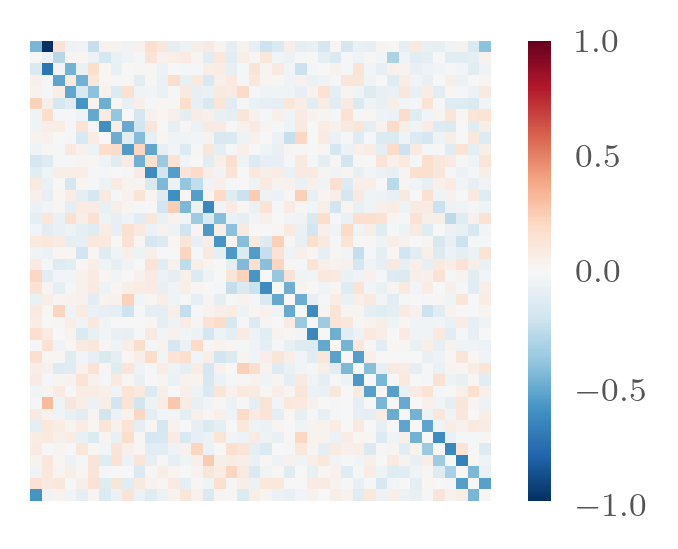
\includegraphics[]{figures/lm_coeff.png}
  \caption{\label{fig:lm_coeff} The coefficient matrix \(\vb{X}\) found from
    least squares linear regression.}
\end{figure}

Applying Ridge regression with different regularization parameters yields
improved results. As seen from~\cref{fig:ridge_coeff}, the penalty sets the
off-diagonal elements closer to zero as we would like. Since Ridge uses
\(L_{2}\) penalty, they do not get set to exactly zero.

\begin{figure}[H]
  \centering
  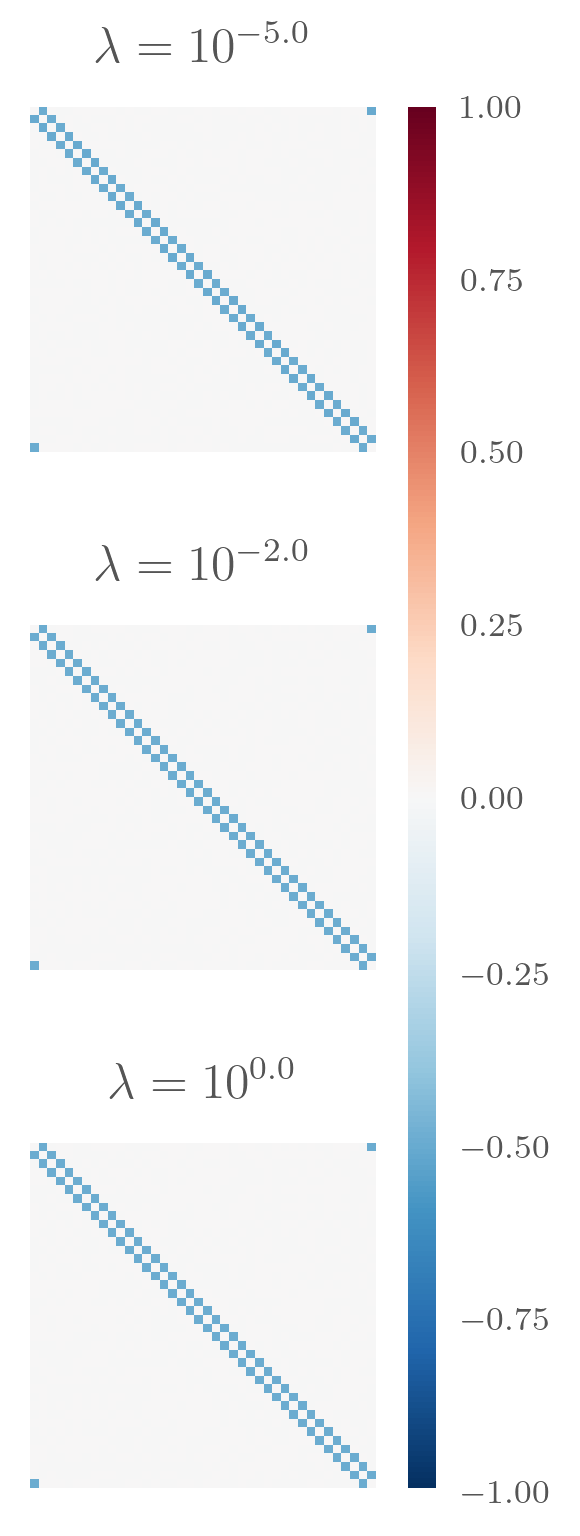
\includegraphics[]{figures/ridge_coeff.png}
  \caption{\label{fig:ridge_coeff} The coefficient matrix \(\vb{X}\) found from
    Ridge regression for different values of regularization parameter. The
    change is so small that it is not noticeable.}
\end{figure}

Lasso behaves differently from the others as it explains all variability using
the upper left triangular part of the coefficient matrix. This is owned to
Lasso's \(L_{1}\) penalization, forcing some coefficients to exactly zero. As
all variability in an \(\{J_{kl}, J_{lk}\}\) pair can be explained by one
coefficient, the other is set to zero, giving only one diagonal. A too large
regularization forces all elements to zero, as seen in the last panel
of~\cref{fig:lasso_coeff},  giving no predictive power.

\begin{figure}[H]
  \centering
  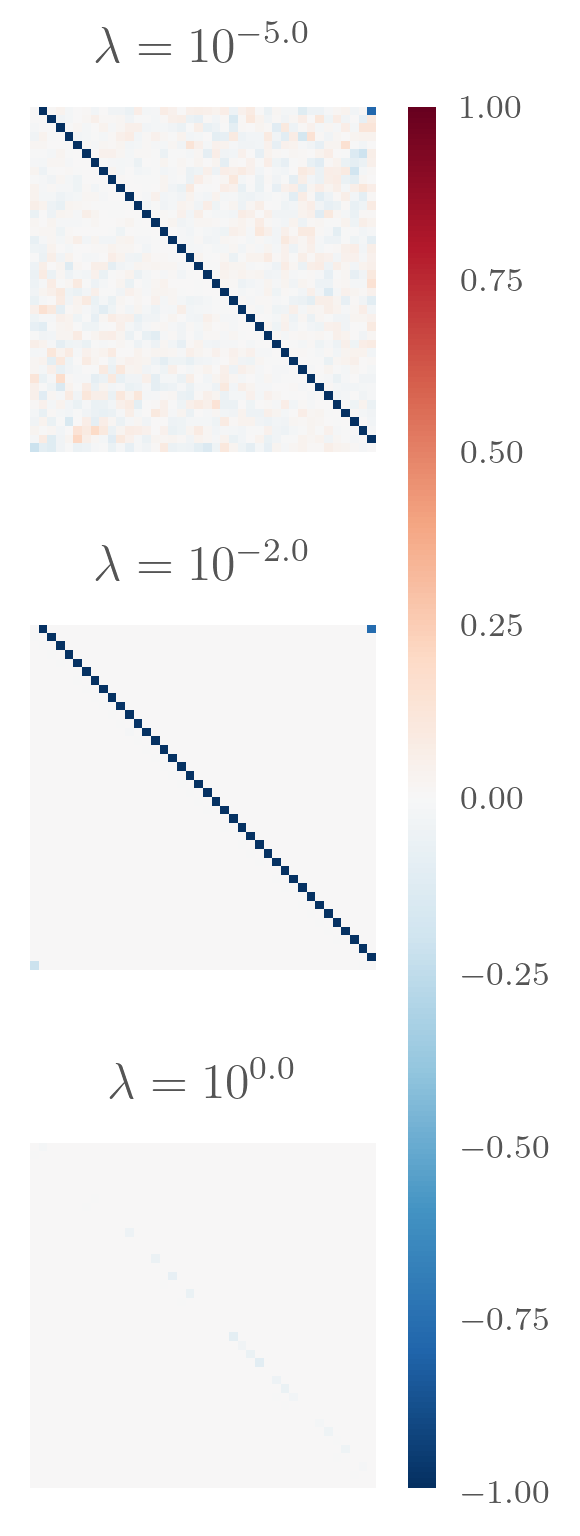
\includegraphics[]{figures/lasso_coeff.png}
  \caption{\label{fig:lasso_coeff} The coefficient matrix \(\vb{X}\) found from
    Lasso regression for different values of regularization parameter. A small
    penalty removes the off-diagonal coefficients, while a too large coefficient
   removes them all.}
\end{figure}

By running a search over log-spaced regularization parameters, the optimal
regularization can be found. This is done for Ridge in~\cref{fig:ridge_reg} and
for Lasso in~\cref{fig:lasso_reg}. The impact on both \(MSE\) and \(R^{2}\) is
shown. Somewhat unexpectedly, the models worsen as the regularization
increases, both for training and test data. The Ridge is very stable over large
ranges, decreasing only for very large regularizations. Lasso
exhibits the same behavior, but dropping quickly to zero as all coefficients are
forced to zero.

The explanation for this is the large number of redundant coefficients in the
model. Only the two off-diagonal lines give non-zero contributions, explaining
all the variance. Once a small regularization is applied, the redundancy is
quickly decreased, decreasing the model variance, and won't decrease again until it is strong enough to affect
the off-diagonal terms, at which point the bias quickly increases.

\begin{figure}[H]
  \centering
  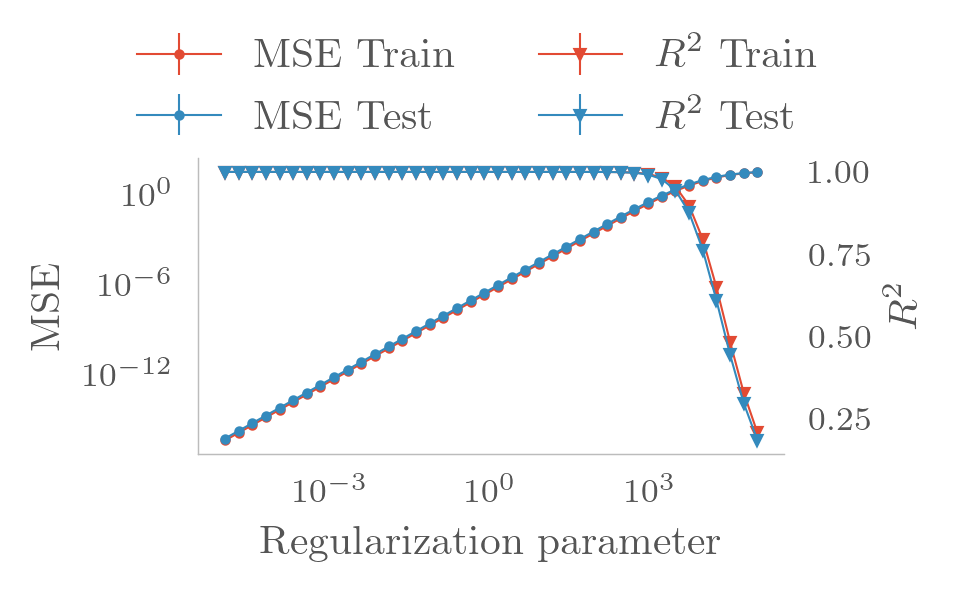
\includegraphics[]{figures/ridge_reg.png}
  \caption{\label{fig:ridge_reg} The mean square error and \(r^{2}\) coefficient
    for Ridge regression with different regularization parameters \(\lambda\)
    from five fold cross validation.
    Any increase in the regularization worsens the performance, as both MSE and
    \(r^{2}\) are monotonically decreasing for the training and test data.}
\end{figure}


\begin{figure}[H]
  \centering
  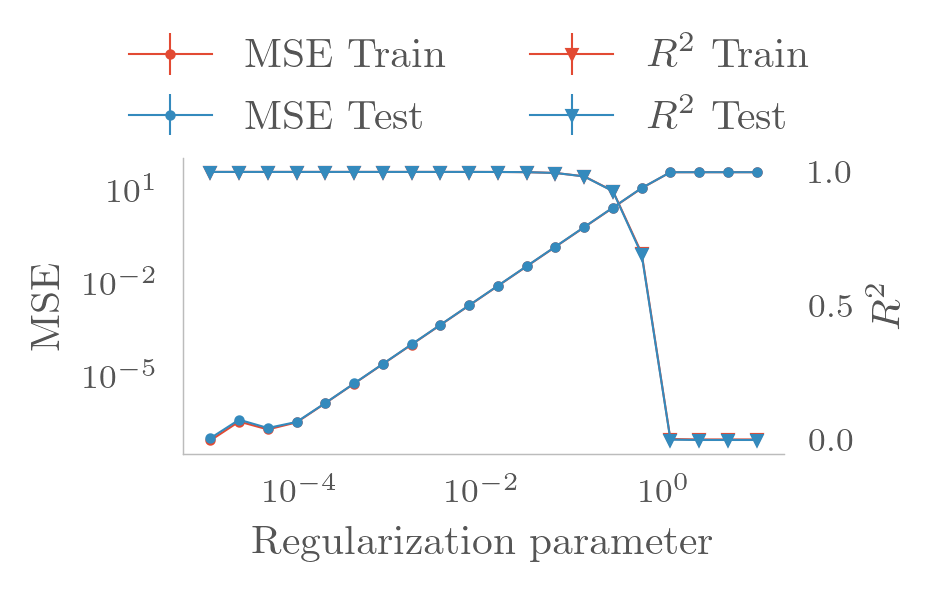
\includegraphics[]{figures/lasso_reg.png}
  \caption{\label{fig:lasso_reg} The mean square error and \(R^{2}\) coefficient
    for Lasso regression with different regularization parameters \(\lambda\)
    from five fold cross validation.
    Any increase in the regularization worsens the performance, as both MSE and
    \(R^{2}\) are monotonically decreasing for the training and test data.}
\end{figure}

\subsubsection{Regression with Neural Nets}

A neural net was trained using a single linear layer on the same data as for the
regression methods. The net was highly sensitive for different learning rates,
so a low rate of \(\eta = 0.0001\) had to be used. Nevertheless, the net quickly
converged, suggesting the weights shown in~\cref{fig:netreg}. Comparing to the
previous results, we see that it is qualitatively identical to least squares and
Ridge, but having off-diagonal less noise than least squares and more than
Ridge. This is expected, as the neural net does not use any regularization.

\begin{figure}[H]
  \centering
  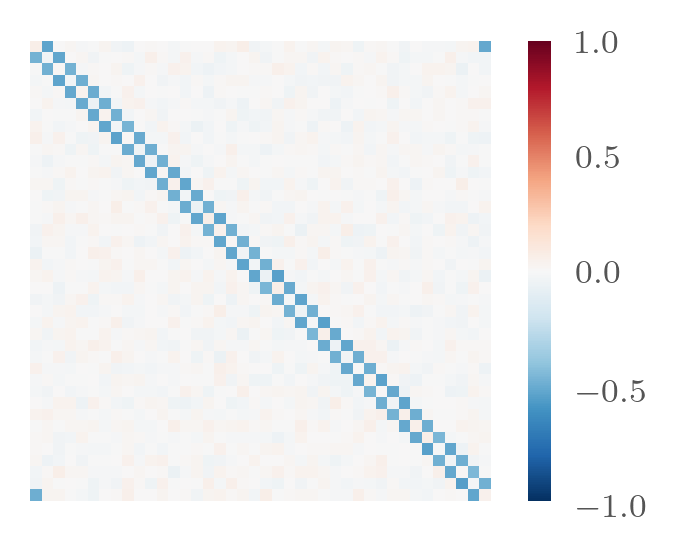
\includegraphics{figures/nnising.png}
  \caption{\label{fig:netreg} The coefficient matrix \(X\) found by neural net.
    The prediction using \(X\) has \(R^{2} = 1.0\) test score.}
\end{figure}


\subsection{Classification}

Classification was performed on ordered and disordered data with \(N=10 000\)
samples. It was discovered that the accuracy score varied wildly depending on which data
was used while cross entropy loss remained nearly constant, but using the whole
data set proved to be too time consuming.

The implementations of normal gradient descent and Nesterov gradient descent
were used together with stochastic descent from \texttt{sklearn}. The behavior
of the former are shown in~\cref{fig:GD_loss}. Both methods overfit the data
quickly, with Nesterov being much faster to overfit. To remedy this, early
stopping was used, causing both to stop after only \(3-10\) iterations. The
results are shown in~\cref{tab:1}.

These results are in agreement with Mehta~\cite{mehta} with test classification
accuracy being around \(50\%\). Since the problem is a binary classification
problem, this is disappointing as it is no better than a random guess.

\begin{figure}[H]
  \centering
  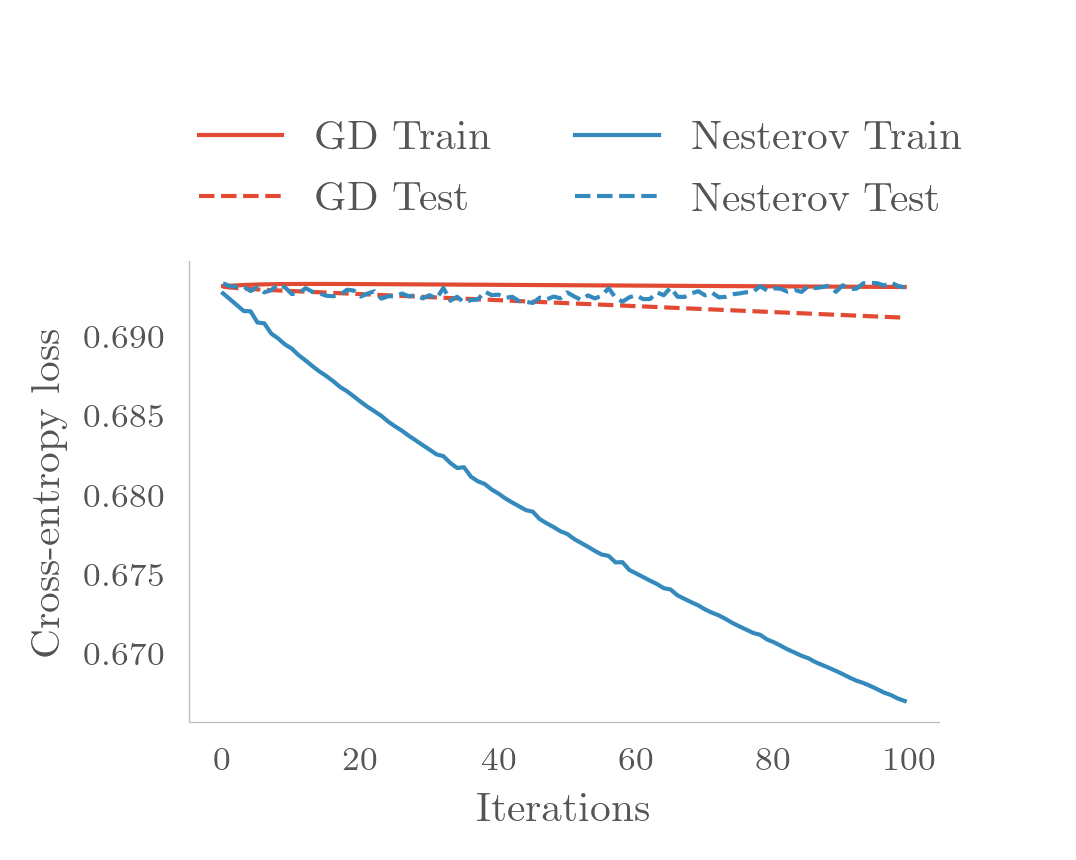
\includegraphics[]{figures/GD_loss.png}
  \caption{\label{fig:GD_loss} The log cross entropy loss for each iteration
    of normal gradient descent and Nesterov gradient descent with learning rate
    \(\eta = 0.001\) for gradient descent and \(\eta = 0.0001\) for Nesterov.
    The Nesterov descent used a batch size \(250\).}
\end{figure}

\begin{table}
  \centering
  \begin{tabular}{l|c|c}
    \multirow{2}{*}{Method} & \multicolumn{2}{c}{Accuracy score}\\
    & Train & Test \\
    \hline
    GD & 0.61 & 0.49 \\
    NGD & 0.51 & 0.70 \\
    SGD & 0.75 & 0.52\\
  \end{tabular}
  \caption{The accuracy score for both training and test data for custom
    implementations of gradient descent and Nesterov descent, as well as
    \texttt{sklearn}'s stochastic gradient descent. The samples were $N=10000$.
    The results varied wildly depending on the data set used.}
  \label{tab:1}
\end{table}


\subsection{Classification With Neural Nets}

While classifying with a logistic classifier has only a handful of
hyperparameters to tune, neural nets have so many that the parameter space can
not be searched within practical time limits. In addition, tuning many
parameters begs for visualizing high dimensional data, which quickly becomes
noisy and uninformative. As such, only learning rates, activation function and
number of hidden neurons were tuned.

Figures~\ref{fig:sigmoid_grid}, \ref{fig:relu_grid} and~\ref{fig:leaky_grid}
show the test accuracy as a function of learning rate \(\eta\) and number of
neurons in the hidden layer for sigmoid, ReLU and leaky ReLU activation
functions. At a glance there are some noticeable differences.

For both ReLU and leaky ReLU, a too high learning rate ends in divergence. The
reason is that the network is taking too large steps and
quickly diverging. However, once the learning rate is low enough, the fast
learning of ReLU's allows for the networks to get high accuracy even with few
neurons. A near perfect test accuracy is achieved with only \(5\) neurons in
both cases. 

The sigmoidal networks behave differently. The best results are achieved at high
learning rates, becoming progressively poorer at lower rates. In addition,
few neurons are preferred. Both of these facts suggest that the network learns
too slowly to fully exploit more neurons, something which is only worsened by
lower learning rates.

\begin{figure}[H]
  \centering
  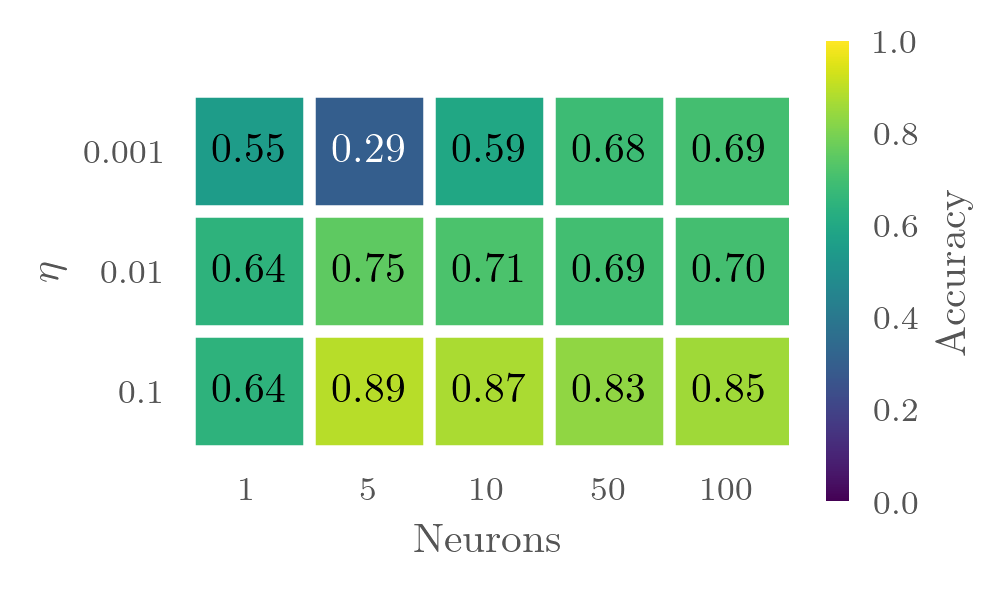
\includegraphics[]{figures/sigmoidgrid.png}
  \caption{\label{fig:sigmoid_grid} The test accuracy of a NN with sigmoid
    activation functions in the hidden layer. The network performs best at high learning
    rates and few neurons. }
\end{figure}

\begin{figure}[H]
  \centering
  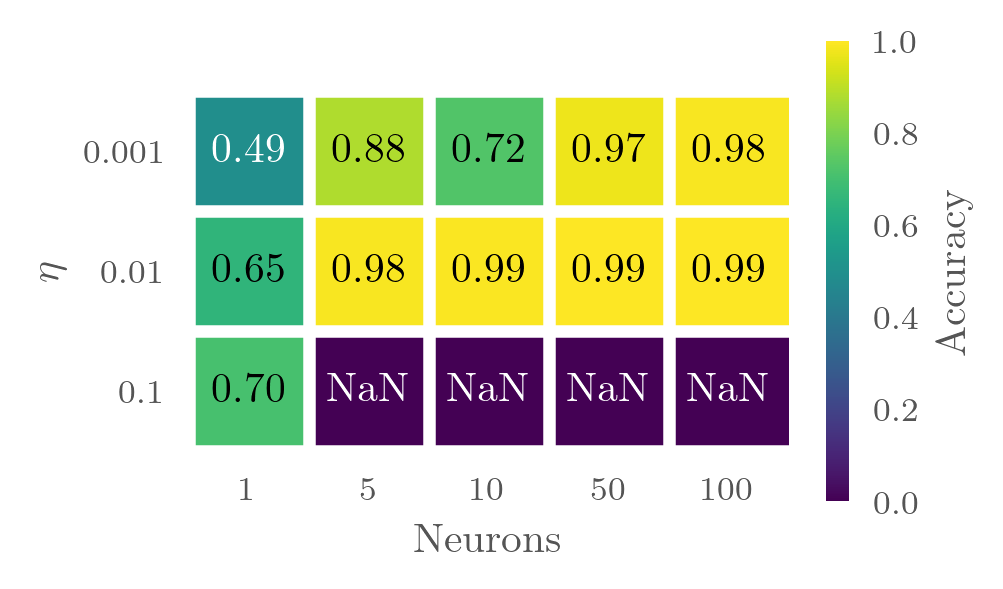
\includegraphics[]{figures/relugrid.png}
  \caption{\label{fig:relu_grid} The test accuracy of a NN with ReLU activation
  functions in the hidden layer. For high learning rates the network diverges.
  Best results are achieved with more than \(1\) neuron and low learning rates.}
\end{figure}

\begin{figure}[H]
  \centering
  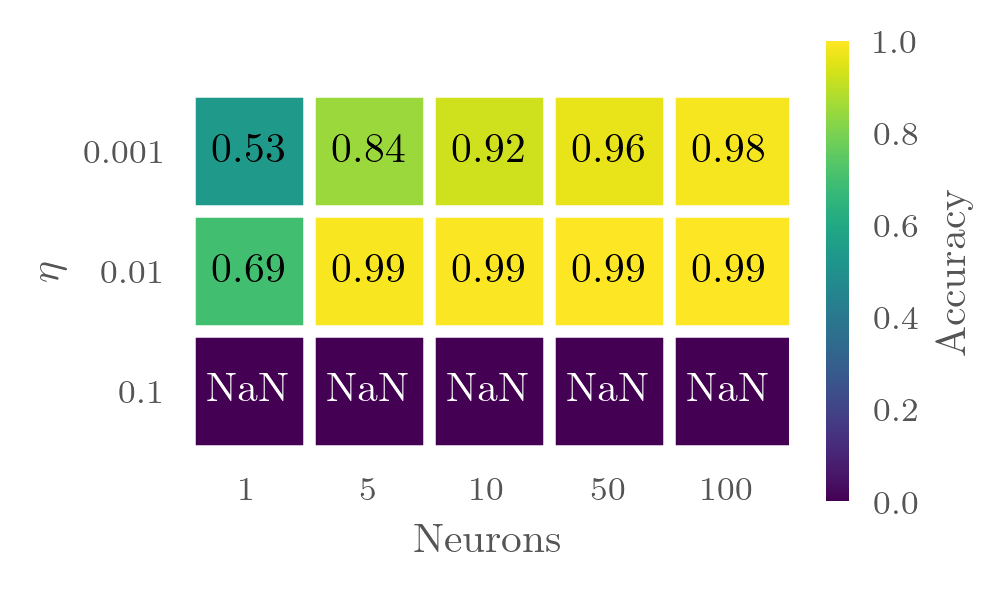
\includegraphics[]{figures/leakygrid.png}
  \caption{\label{fig:leaky_grid} The test accuracy of a NN with leaky ReLU
    activation functions in the hidden layer. Diverges for too high learning
    rates, while achieved nearly perfect accuracy for all other cases.}
\end{figure}

The near perfect learning rates are at first sight dubious, but this is
consistent with independent analyses, most notably Mehta et al.\cite{mehta}. It
is neither an unreasonable result, as the classification problem is binary with
predictors of equal variance. There is also the additional benefit that random
data can be classified as unordered systems, as this would indeed be correct. In
other words, the network does not need to learn what unordered systems look
like, only what ordered systems look like, as everything that is not ordered, be
it ``real'' unordered systems or random data, are indistinguishable from unordered.

In total, using ReLU or leaking ReLU with low learning rates and a few neurons
gives optimal results with the least computational demand. The classification
was not tested in the critical regime, something which should be performed in
future work. 
